\chapter{Modelli e Funzionamento}\label{cap:modefunz}
\section{Blazor Server}\label{sez:bserver}
Il primo dei modelli ufficialmente rilasciati e per il quale si pu\'o ricevere supporto in produzione da settembre 2019\cite{blazorServerRelease}, \'e proprio questo.

Un'applicazione Blazor Server ospita i componenti Blazor lato Server e gestisce le interazioni dell'utente con la UI attraverso una connessione in tempo reale sfruttando SignalR, come visibile nella figura 2.1.

\begin{figure}[H]
	\centerline{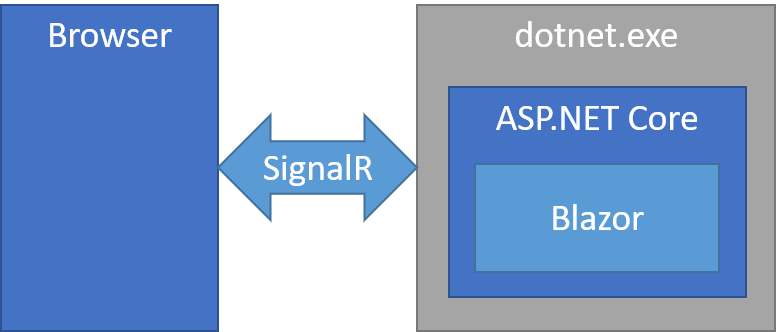
\includegraphics[scale=0.6]{figure/blazor-server.png}}
	\caption{Blazor Server}
	\label{fig:BlazorServer}
\end{figure}

Quando un utente scatena un evento, questo viene inviato attraverso la RTC al server, dove i vari componenti gestiscono l'evento.
Quando l'evento \'e stato gestito, blazor compara l'output generato con quello precedente l'evento, e manda quindi le sole differenze al browser del client, per poi applicarle al DOM.\cite{blazorModelsScenarios}

Blazor Server quindi necessita di una connessione stabile e a bassa latenza per funzionare al meglio, e gli scenari offline non sono supportati.

\'E particolarmente indicato quando si vuole delegare il costo computazionale al server e non ai client connessi, dato che ci\'o che il client esegue \'e il solo codice statico e le differenze di volta in volta inviate ma calcolate lato server.
Ci\'o rende molto veloce ed efficiente l'avvio dell'applicazione e in particolare il suo caricamento iniziale lato client, che rende il modello perfetto per funzionare su apparecchi a basso costo.
\pagebreak
%Oltretutto ci\'o che viene scaricato lato client non varia al crescere dell'applicazione lato server.

\section{Blazor WebAssembly}\label{sez:bclient}
Blazor WebAssembly \'e un modello attualmente in preview, che verr\'a ufficialmente rilasciato nella prima parte del 2020.

In questo modello il codice della SPA viene eseguito completamente lato client come solitamente avviene quando si utilizza un framework moderno per UI basato su JS, come i gi\'a citati Angular,React,Vue.

\begin{figure}[H]
	\centerline{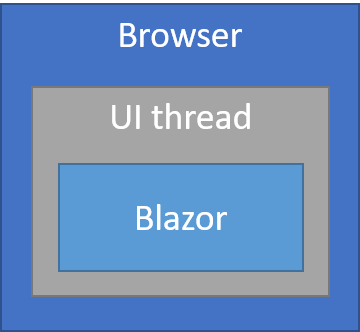
\includegraphics[scale=0.6]{figure/blazor-webassembly.png}}
	\caption{Blazor Webassembly}
	\label{fig:BlazorWebassembly}
\end{figure}

Vengono quindi scaricati dal client l'applicazione Blazor, le sue dipendenze, ed il runtime del .NET scelto come target per l'applicazione.
L'applicazione viene quindi eseguita direttamente nel thread della User Interface del Browser utilizzato, come visibile nella figura 2.2.

Quindi esegue nella stessa sandbox di qualsiasi altra applicazione javascript, e non pu\'o fare niente di pi\'u o di meno. Ogni update alla UI e la gestione di ciascuno, avvengono utilizzando lo stesso processo nel browser. Per questo modello, blazor.webassembly.js \'e il nome dello script Javascript che si occupa di scaricare il .NET runtime, l'applicazione e le dipendenze, come anche dell'inizializzazione dell'applicazione. 
In particolare il nome Blazor WebAssembly \'e stato scelto perch\'e il WebAssembly \'e il byte code del web che dal 2015 i browser pi\'u diffusi al mondo si sono impegnati per sviluppare ed adottare.
\pagebreak

\section{Blazor PWA}\label{sez:bpwa}
Lo step successivo per avvicinarsi al client allontanandosi dal modello server \'e poi Blazor PWA.

\'E cos\'i chiamato perch\'e in questo modello Blazor, permette di sviluppare l'interfaccia utente di una Progressive Web App.
Nella figura 2.3 viene riassunto cosa sia una Progressive Web App.

\begin{figure}[H]
	\centerline{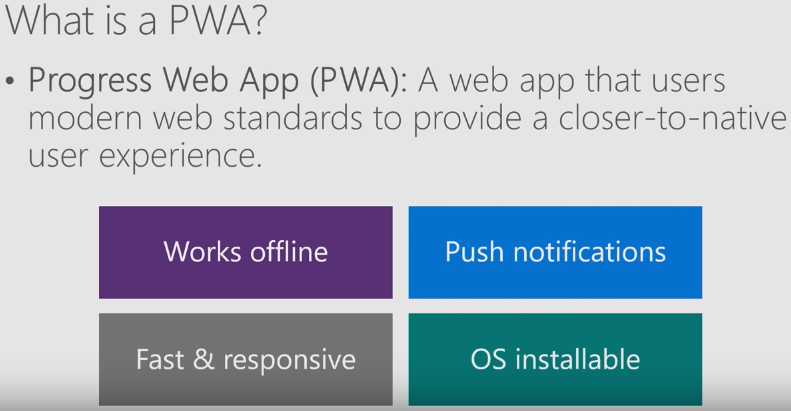
\includegraphics[scale=0.5]{figure/ProgressiveWebApp.png}}
	\caption{Progressive Web Apps}
	\label{fig:WhatIsAPWA}
\end{figure}


In particolare queste sono applicazioni web che hanno la capacit\'a di funzionare anche offline, e che spesso possono essere scaricate in modo persistente sulla macchina dell'utente che le esegue.
Offrono chiaramente una maggiore velocit\'a di esecuzione e la possibilit\'a di sfruttare alcune API native.
Ad esempio possono essere utilizzate quando la necessit\'a \'e quella di utilizzare le notifiche push native del SO che sta utilizzando il client(e.g. Windows).

Per realizzarne una in Blazor al momento, bisogna partire dal modello Blazor WebAssembly aggiungendo un manifesto che descriva le capacit\'a dell'applicazione, i permessi richiesti e l'icona da utilizzare una volta installata, oltre chiaramente a dover implementare l'applicazione in modo che possa lavorare anche offline, basandosi su un service worker.\cite{blazorPWA}
\pagebreak

\section{Blazor Hybrid}\label{sez:bhybrid}
Da questo punto in poi, i modelli di Blazor servono a sviluppare applicazioni native.
Nel modello Hybrid, l'applicazione sviluppata non \'e quindi pi\'u considerabile una web app ma rimane ibrida perch\'e pur essendo un app nativa, utilizza tecnologie web per effettuare il rendering della user interface.

Esempi di Hybrid Apps possono essere applicazioni mobile native, che hanno accesso alle API esposte ad esempio da Android, ma che utilizzano delle WebViews per la gestione dell'interazione dell'utente con la UI.

Un'altro esempio molto interessante sono le applicazioni che sfruttano Electron, che permette di compilare un'applicazione web in un applicazione desktop cross platform.
Infatti utilizzando Electron si pu\'o creare un'applicazione nativa, con l'interfaccia utente scritta utilizzando blazor, facendo in modo che in fase di esecuzione il processo host sia .NET Core(avendo quindi pieno accesso alle capacit\'a native e ad esempio al file system) pur rimanendo cross platform e potendo quindi eseguire su Windows, Linux e Mac.
Di seguito nell'immagine 2.4 si pu\'o vedere una Web Application compilata nativamente con Electron(con target Windows), e quindi eseguita come applicazione desktop:

\begin{figure}[H]
	\centerline{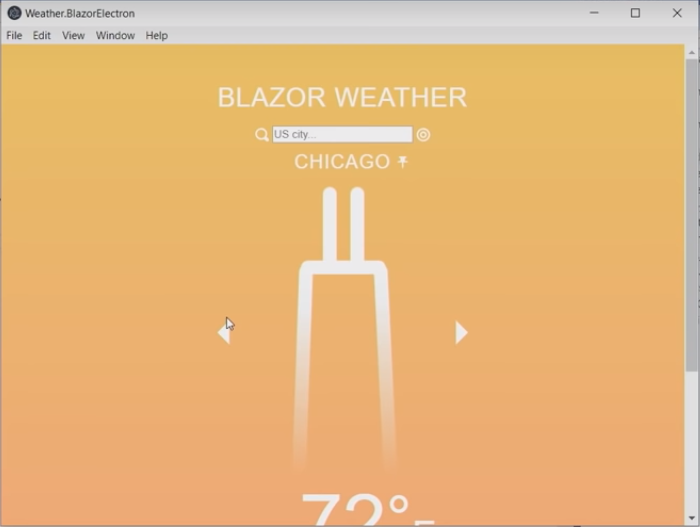
\includegraphics[scale=0.6]{figure/BlazorWeatherElectron.png}}
	\caption{Blazor Hybrid Application}
	\label{fig:BlazorHybridApplication}
\end{figure}

Il codice open source dell'applicazione qui sopra, si trovare al seguente link: https://github.com/danroth27/BlazorWeather/tree/master/BlazorWeather.Electron
\pagebreak



\section{Blazor Native}\label{sez:bnative}
Infine esiste il modello Native che \'e possibile grazie al fatto che Blazor \'e stato architettato per poter renderizzare controlli della User Interface che non siano obbligatoriamente strumenti web, e pu\'o quindi integrarsi con controlli nativi.
Il rendering layer \'e infatti intercambiabile, pur essendo quello di default dedicato all'HTML.

Un esempio di applicazione sviluppata utilizzando Blazor per il rendering di controlli nativi nella user interface, si pu\'o vedere durante la presentazione di Steve Sanderson all' evento NDC Oslo di quest'anno, pur non essendo stato ancora rilasciato il codice di un esempio ufficiale.\cite{sandersonNDCBlutter}
In questa applicazione, si \'e scelto di sostituire il default rendering layer per utilizzarne uno custom, utilizzando componenti di Flutter, il toolkit di Google per costruire interfacce utente native CrossPlatform.
Questo modello viene qui citato per completezza, ma al momento non \'e nemmeno presente nella documentazione ufficiale ed \'e solo stato citato da Daniel Roth durante la presentazione dei futuri modelli di Blazor lato client.\cite{blazorNative}
\pagebreak